\section{Results and Analysis}

\subsection{Main EuroSAT Results}
Table~\ref{tab:eurosat-main} reports overall accuracy across all five modality configurations on EuroSAT. Houlsby adapters dominate every modality, while standard LoRA tracks the linear-probe baseline within $\pm 0.001$ OA --- consistent with complete failure under the original implementation. The split-QKV ablation recovers most of LoRA's expected gain on s2\_full but, as analyzed below, still falls short of both BitFit and Houlsby.

\begin{table}[t]
\centering
\small
\caption{EuroSAT~\cite{helber2019eurosat} overall accuracy across five modality configurations. Mean $\pm$ std over three seeds; full fine-tuning is reported as a single run. Best PEFT result per column in \textbf{bold}.}
\label{tab:eurosat-main}
\begin{tabular}{lccccc}
\toprule
Method & s2\_full & rgb & rgb\_sar & gf2 & sar\_only \\
\midrule
Linear Probe        & 0.657 $\pm$ 0.002 & 0.556 $\pm$ 0.004 & 0.552 $\pm$ 0.002 & 0.649 $\pm$ 0.006 & 0.387 $\pm$ 0.004 \\
BitFit              & 0.702 $\pm$ 0.002 & 0.608 $\pm$ 0.001 & 0.605 $\pm$ 0.002 & 0.701 $\pm$ 0.001 & 0.449 $\pm$ 0.003 \\
LoRA (r=8)          & 0.658 $\pm$ 0.003 & 0.556 $\pm$ 0.003 & 0.553 $\pm$ 0.003 & 0.650 $\pm$ 0.006 & 0.388 $\pm$ 0.004 \\
LoRA Split-QKV      & 0.707 $\pm$ 0.003 & 0.498 $\pm$ 0.006 & --- & --- & --- \\
Houlsby             & \textbf{0.821 $\pm$ 0.003} & \textbf{0.727 $\pm$ 0.003} & \textbf{0.738 $\pm$ 0.002} & \textbf{0.820 $\pm$ 0.002} & \textbf{0.615 $\pm$ 0.004} \\
GeoAdapter v2       & 0.485 $\pm$ 0.056 & 0.383 $\pm$ 0.015 & --- & --- & --- \\
\midrule
Full Fine-Tuning    & 0.869 & --- & --- & --- & --- \\
\bottomrule
\end{tabular}
\end{table}

Two patterns are immediately visible. (i)~The Houlsby--linear-probe gap is consistent across modalities ($+16.4\%$ to $+22.8\%$ OA), suggesting the gain is structural rather than modality-specific. (ii)~The cross-modality gap dominates the cross-method gap whenever the spectral input is degraded: switching from s2\_full to sar\_only costs more accuracy (e.g.~$-20.6\%$ for Houlsby) than switching between PEFT methods at fixed modality.

\subsection{Main BigEarthNet Results}
Table~\ref{tab:bigearthnet-main} validates the EuroSAT ranking on a larger, multi-label benchmark. Houlsby again leads, while LoRA and linear probing are statistically indistinguishable.

\begin{table}[t]
\centering
\caption{BigEarthNet-S2~\cite{sumbul2019bigearthnet} validation mAP (19-class multi-label, mean $\pm$ std over three seeds).}
\label{tab:bigearthnet-main}
\begin{tabular}{lcc}
\toprule
Method & s2\_full & rgb \\
\midrule
Linear Probe & 0.358 $\pm$ 0.003 & 0.335 $\pm$ 0.001 \\
LoRA (r=8) & 0.358 $\pm$ 0.003 & 0.335 $\pm$ 0.001 \\
Houlsby & \textbf{0.491 $\pm$ 0.008} & \textbf{0.456 $\pm$ 0.003} \\
\bottomrule
\end{tabular}
\end{table}

\subsection{Finding 1: Why LoRA Fails}
The naive LoRA result initially suggested complete failure: on EuroSAT, LoRA differs from linear probing by only $+0.001$ OA, and on BigEarthNet-S2 by only $+0.0001$ mAP. Our split-QKV ablation reveals that this failure has two distinct causes.

First, the standard implementation misses the actual query, key, and value projections because Prithvi's attention stores them as a fused \texttt{in\_proj\_weight} parameter rather than as separate child modules. As a result, the original LoRA insertion only wraps \texttt{out\_proj}. Second, even when the fused QKV issue is corrected, LoRA remains suboptimal. Split-QKV LoRA improves s2\_full from 0.658 to 0.707 on EuroSAT, confirming the implementation trap is real, but it still underperforms both BitFit and Houlsby. On rgb, split-QKV LoRA actually degrades below the linear probing baseline.

Together, these observations show that LoRA fails on Prithvi-100M not only because of an implementation pitfall, but also because low-rank adaptation appears mismatched to this architecture and pre-training regime. We further validated this point with a rank-sensitivity ablation on EuroSAT s2\_full (Figure~\ref{fig:lora-rank}): increasing the split-QKV LoRA rank from $r=4$ to $r=32$ changes OA only from $0.709 \pm 0.002$ to $0.706 \pm 0.002$, with no monotonic improvement and no configuration approaching Houlsby.

\begin{figure}[t]
\centering
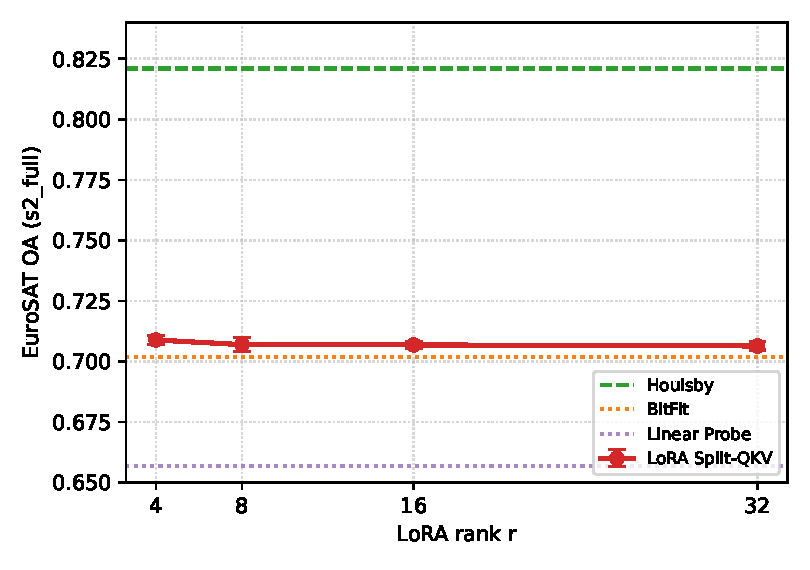
\includegraphics[width=0.78\linewidth]{figures/lora_rank_sensitivity.pdf}
\caption{Split-QKV LoRA rank sensitivity on EuroSAT s2\_full. Raising the rank from 4 to 32 does not materially improve accuracy, indicating that the post-fix LoRA ceiling is not explained by an underpowered rank choice.}
\label{fig:lora-rank}
\end{figure}

\subsection{Finding 2: Houlsby Consistently Dominates}
Houlsby adapters are the best method on every evaluated configuration. On EuroSAT, they outperform linear probing by $+16.4\%$ to $+22.8\%$ OA depending on modality. On BigEarthNet-S2, they outperform linear probing by $+13.3$ mAP on s2\_full and $+12.1$ mAP on rgb. This consistency across datasets and tasks is the strongest empirical conclusion of the benchmark. The full fine-tuning baseline further clarifies the quality of this result: full fine-tuning reaches 0.869 OA on EuroSAT s2\_full while Houlsby reaches 0.821, corresponding to 94.5\% of the full fine-tuning score with only 1.4\% of the trainable parameters (Figure~\ref{fig:acc-vs-params}).

\begin{figure}[t]
\centering
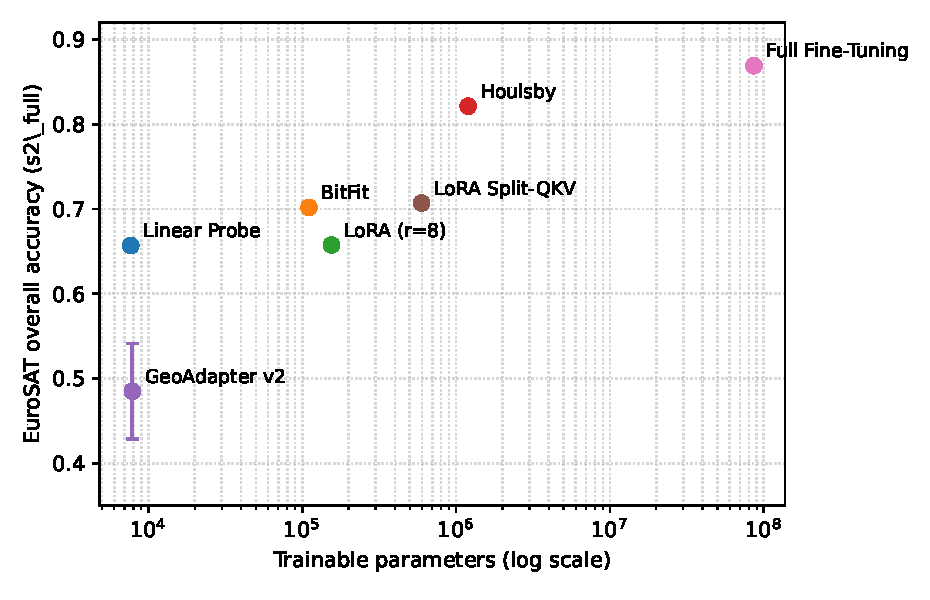
\includegraphics[width=0.78\linewidth]{figures/acc_vs_params.pdf}
\caption{EuroSAT s2\_full overall accuracy versus trainable parameter count (log scale). Houlsby adapters reach 94.5\% of the full fine-tuning ceiling using 1.4\% of the parameters; standard LoRA collapses to the linear-probe baseline.}
\label{fig:acc-vs-params}
\end{figure}

\subsection{Finding 3: Modality Selection Matters More Than Method Selection}
Across both datasets, richer spectral inputs consistently outperform reduced-band subsets. On BigEarthNet-S2, the s2\_full--rgb gap is $+0.023$ mAP for linear probing, $+0.023$ mAP for LoRA, and $+0.035$ mAP for Houlsby. On EuroSAT (Figure~\ref{fig:per-modality}), the spread between modalities is even larger: switching from s2\_full to sar\_only costs Houlsby $-20.6\%$ OA, more than the entire spread between BitFit and Houlsby on s2\_full.

\begin{figure}[t]
\centering
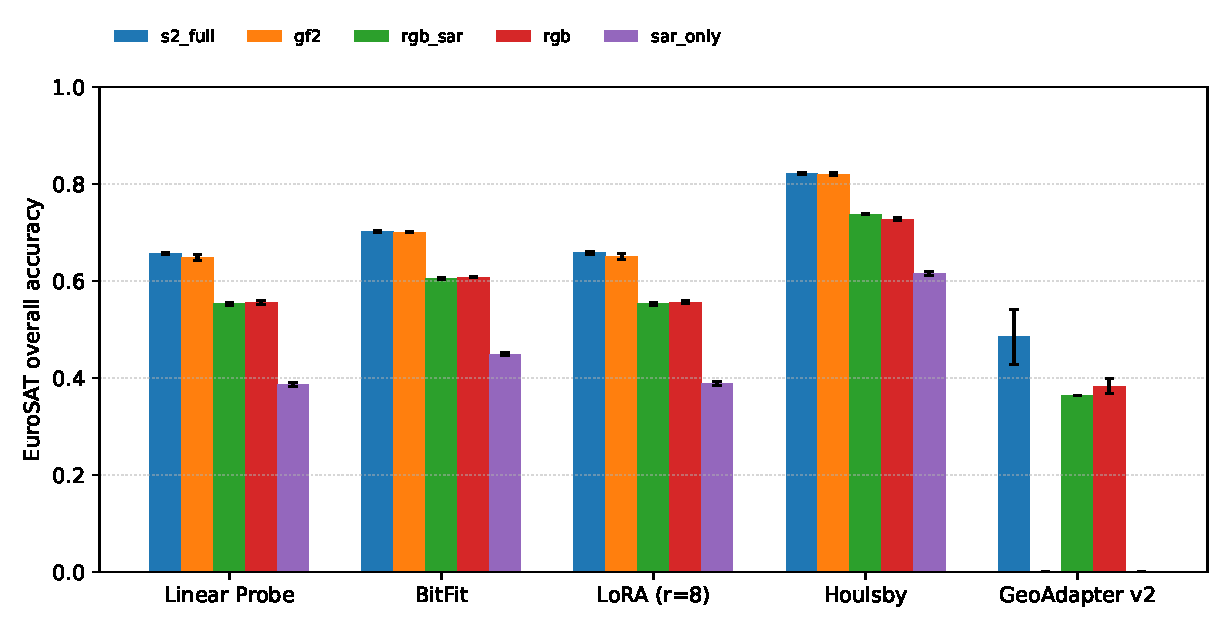
\includegraphics[width=0.92\linewidth]{figures/per_modality_oa.pdf}
\caption{EuroSAT overall accuracy per modality, grouped by PEFT method. Modality selection (color groups) shifts OA more than method selection (within-group ordering) for every method except linear probing.}
\label{fig:per-modality}
\end{figure}

This result suggests that practitioners should first maximize input information quality before worrying about subtle PEFT differences. A simple linear probe on better spectral inputs can outperform more sophisticated adaptation on weaker input subsets.

\subsection{Finding 4: Input-Stage Adaptation Remains a Negative Result}
GeoAdapter v2 consistently underperforms the linear probing baseline on EuroSAT. Although it was designed to bridge modality mismatches at the input stage, its residual adapter structure does not provide a stable optimization path under a frozen transformer backbone. The high seed variance on s2\_full ($\pm 0.056$) is itself diagnostic: the optimization landscape is unstable, and the negative result therefore reflects a structural rather than a hyperparameter issue. We conclude that modality adaptation is more effectively handled by backbone-level PEFT than by a tiny standalone input bridge.

\subsection{Practical Takeaways}
The benchmark supports three practical recommendations. First, Houlsby adapters are the safest default for adapting Prithvi-100M to heterogeneous inputs. Second, LoRA should not be assumed effective in GeoFMs without careful architectural inspection. Third, when spectral richness is available, preserving that information has larger returns than switching between weak PEFT methods.
